% id: 91-02
% book: 개념원리 중학 3-2 · 09 원주각
% section: 이런 문제가 시험에 나온다
% figure: crop:fig-91-02.png
% answer: $5\pi\mkern3mu \mathrm{cm}^2$
% answer_source: 답지
% variant_level: 0 (원본 전사)
% 이 파일은 build.mjs 가 items.json 에서 만든다. 고칠 때는 items.json 을 고친다.
\smash{\raisebox{1.5mm}{\dmkichul{개념원리 중학 3-2 91쪽 02번}}}
\noindent\begin{minipage}[t]{0.58\linewidth}\vspace{0pt}\raggedright 오른쪽 그림과 같이 반지름의 길이가 $3\mkern3mu \mathrm{cm}$인 원~$\pt{O}$에서 $\angle\pt{ABC}=100^\circ$일 때, 색칠한 부분의 넓이를 구하시오.\end{minipage}\hfill\begin{minipage}[t]{0.4\linewidth}\vspace{0pt}\centering \setlength{\dmfigw}{77.4pt}\ifdim\dmfigw>\linewidth\setlength{\dmfigw}{\linewidth}\fi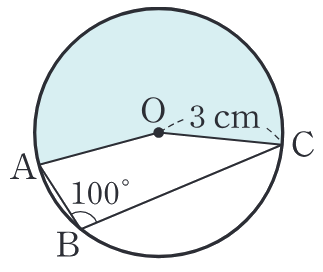
\includegraphics[width=\dmfigw]{figures/fig-91-02.png}\end{minipage}\par
